
%(BEGIN_QUESTION)
% Copyright 2007, Tony R. Kuphaldt, released under the Creative Commons Attribution License (v 1.0)
% This means you may do almost anything with this work of mine, so long as you give me proper credit

Identify all the components shown in this P\&ID of an analog flow control system:

$$\includegraphics[width=15.5cm]{i02423x01.eps}$$

\vskip 10pt

Identify all the components shown in this P\&ID of the same flow control loop implemented using a DCS:

$$\includegraphics[width=15.5cm]{i02423x02.eps}$$

\vskip 10pt

\filbreak

Identify all the components shown in this P\&ID of the same flow control loop implemented using a device-level fieldbus and a DCS:

$$\includegraphics[width=15.5cm]{i02423x03.eps}$$

\vskip 10pt

Finally, identify all the components shown in this P\&ID of the same flow control loop implemented entirely with a device-level fieldbus:

$$\includegraphics[width=15.5cm]{i02423x04.eps}$$

In each of these control systems, identify where the control algorithm (PID calculations) take place.

\vskip 20pt \vbox{\hrule \hbox{\strut \vrule{} {\bf Suggestions for Socratic discussion} \vrule} \hrule}

\begin{itemize}
\item{} How are Fieldbus signal paths represented using ISA-standard symbols in P\&IDs?
\item{} What is the distinction in ISA-standard symbology between circles that are filled (solid black) versus circles that are unfilled, when those circles appear as part of a line symbol?
\end{itemize}

\underbar{file i02423}
%(END_QUESTION)





%(BEGIN_ANSWER)

In the analog control system, the PID calculations take place in a front-panel mounted controller in the main control room area.  In the DCS systems, the PID calculations take place in the DCS controller, which is located in some auxiliary location, behind the panel.  In the pure fieldbus system, control takes place in the flow transmitter itself.

\vskip 10pt

Follow-up question: what purpose is served by the ``bridge'' device in the last system?

%(END_ANSWER)





%(BEGIN_NOTES)

In the analog and first two DCS-based systems, all control decisions take place in the FIC (Flow Indicating Controller).  Only in the FOUNDATION Fieldbus system is it possible for control decisions to take place inside the field devices themselves.

\vskip 10pt

Note the different line types: 

\begin{itemize}
\item{} Dashed = analog (4-20 mA) signaling
\item{} Hollow circles = data link (common system, such as within a DCS)
\item{} Hollow circles on dashed = analog with smart communications
\item{} Solid circles = data link (independent systems)
\item{} Hollow diamonds = Fieldbus network
\end{itemize}

\vskip 10pt

The bridge device interfaces the device-level fieldbus with the control network where the flow recorder resides.

%INDEX% Fieldbus, control: functions residing in devices rather than centralized controller

%(END_NOTES)


